\documentclass[12pt,letterpaper]{article}
\usepackage{lipsum}
\usepackage{amssymb}
\usepackage{amsmath}
\usepackage{graphicx}
\graphicspath{ {} }
\usepackage{authblk}
\usepackage[top=0.8in, bottom= 0.8in, left= 0.8in, right= 0.8in]{geometry}
\usepackage{fancyhdr}

\pagestyle{fancy}
\begin{document}

%title and author details
\title{Laboratory III, Problem I: Forces and Motion}
\author[]{Cole Nielsen}
\date{October 20, 2014} 
\affil[]{Physic 1301W TA: Yao Meng}
\pdfpagewidth 8.5in
\pdfpageheight 11in
%
%
\maketitle
%
\abstract{A cart was connected by pulley and string to a mass hanging at height \(h\) above the ground. The system was allowed to go into motion from its initial state of rest. The cart's motion was recorded using a camera and was analyzed using Motionlab software to find its final velocity. That data was then used to validate a predicted equation that found the final velocity of the cart from the system's intitial conditions. }

\section{Introduction}
The scenario shown below in \textit{Figure 1} was considered. In this scenario, several children at a summer camp have constructed carts to be raced on level surface like shown in \textit{Figure 1}. In order to give each cart a fair start, they are connected by pulley and string to a hanging mass height \(h\) above the ground that accelerates the cart. The system initially starts at rest, and is then allowed to go into motion as a result of acceleration due to gravity acting on the hanging mass. The system will continue to accelerate until the hanging mass has traveled the whole distance of \(h\). Following that, the cart will be free to travel at a constant velocity \(v_f\) equal to the speed of the system the instant before the hanging mass hit the ground.
\newline
\begin{center}
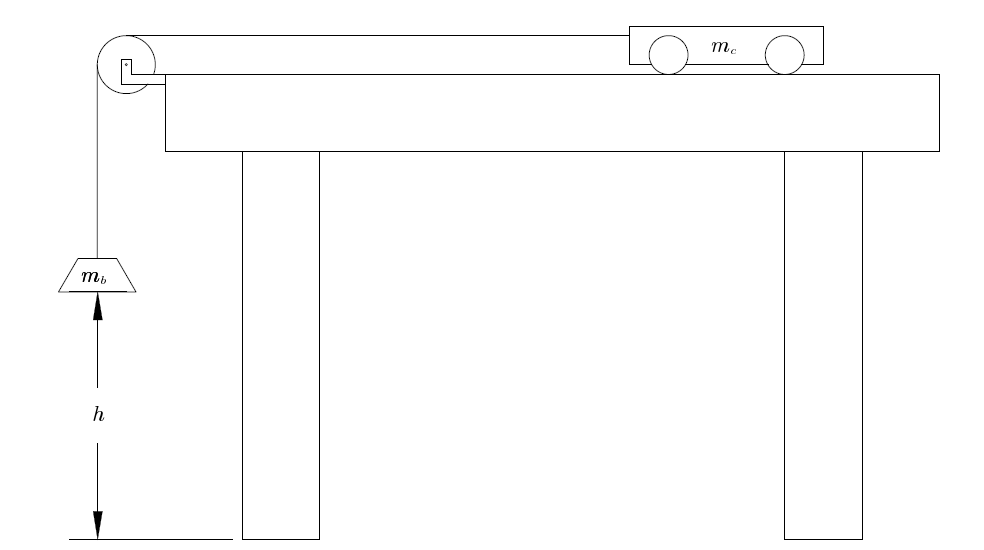
\includegraphics[scale=0.4]{setup.PNG}
\newline\newline
\textit{Figure 1.} The experimental setup.
\end{center}%
\newpage%
In order to predict the winner of the race, a formula has been derived (see the below \textit{Prediction} section) to calculate the final velocity of the cart given the system in \textit{Figure 1's} initial conditions. The initial conditions are as follow: (A) the mass of the cart \(m_c\) (B) the mass of the hanging mass or "basket" \(m_b\) and (C) the hanging mass \(m_b\)'s initial height \(h\). The predicted equation, however, is unproven, so in order to affirm its validity, it must first be tested. This experiment therefore seeks to test and confirm the validity of our predicted equation for \(v_f\).
\section{Prediction}
It is predicted that the final velocity of the cart will be as follows:
\begin{equation}
v_f = \sqrt{2h\frac{m_b g}{m_b + m_c}} 
\end{equation}
Where \(v_f\) is in \(\frac{m}{s}\), \(h\) is in meters, \(m_b\) and \(m_c\) are in kilograms and g is assumned to be equal to acceleration due to gravity near earths surface at 9.81 \(\frac{m}{s^2}\). This equation was derived as follows using kinematic equations and Newton's second law:
\begin{equation}
v_f^2 - v_i^2 = 2 a \Delta x, \hspace{0.25in} v_f^2 = 0, \hspace{0.25in} \Delta x = h  
\end{equation}
\begin{equation}
\therefore \hspace{0.1in} v_f = \sqrt{2ah}
\end{equation}
\begin{equation}
\Sigma F = F_{g,b} = m_b g, \hspace{0.25in} a = \frac{\Sigma F}{\Sigma m}, \hspace{0.25 in} \Sigma m = m_b + m_c
\end{equation}
\begin{equation}
\therefore \hspace{0.1in} a = \frac{m_b g}{m_b + m_c} 
\end{equation}
\begin{equation}
Thus,\hspace{0.1in} v_f =\sqrt{2h \frac{m_b g}{m_b + m_c}} 
\end{equation}
From this equation it can be predicted how each variable \(h\), \(m_b\) and \(m_c\) affects \(v_f\). This is done by choosing one of the variables to test and subsituting all others with constants. Below are the  functions for how each variable affects \(v_f\) and the corresponding graph for each function
\begin{equation}
\hspace{0.3in}v_f(h) = \sqrt{h} \hspace{1.0in} v_f(m_b) = \sqrt{\frac{m_b}{1 + m_b}}\hspace{0.9in} v_f(m_c) = \sqrt{\frac{1}{m_c}}\nonumber
\end{equation}
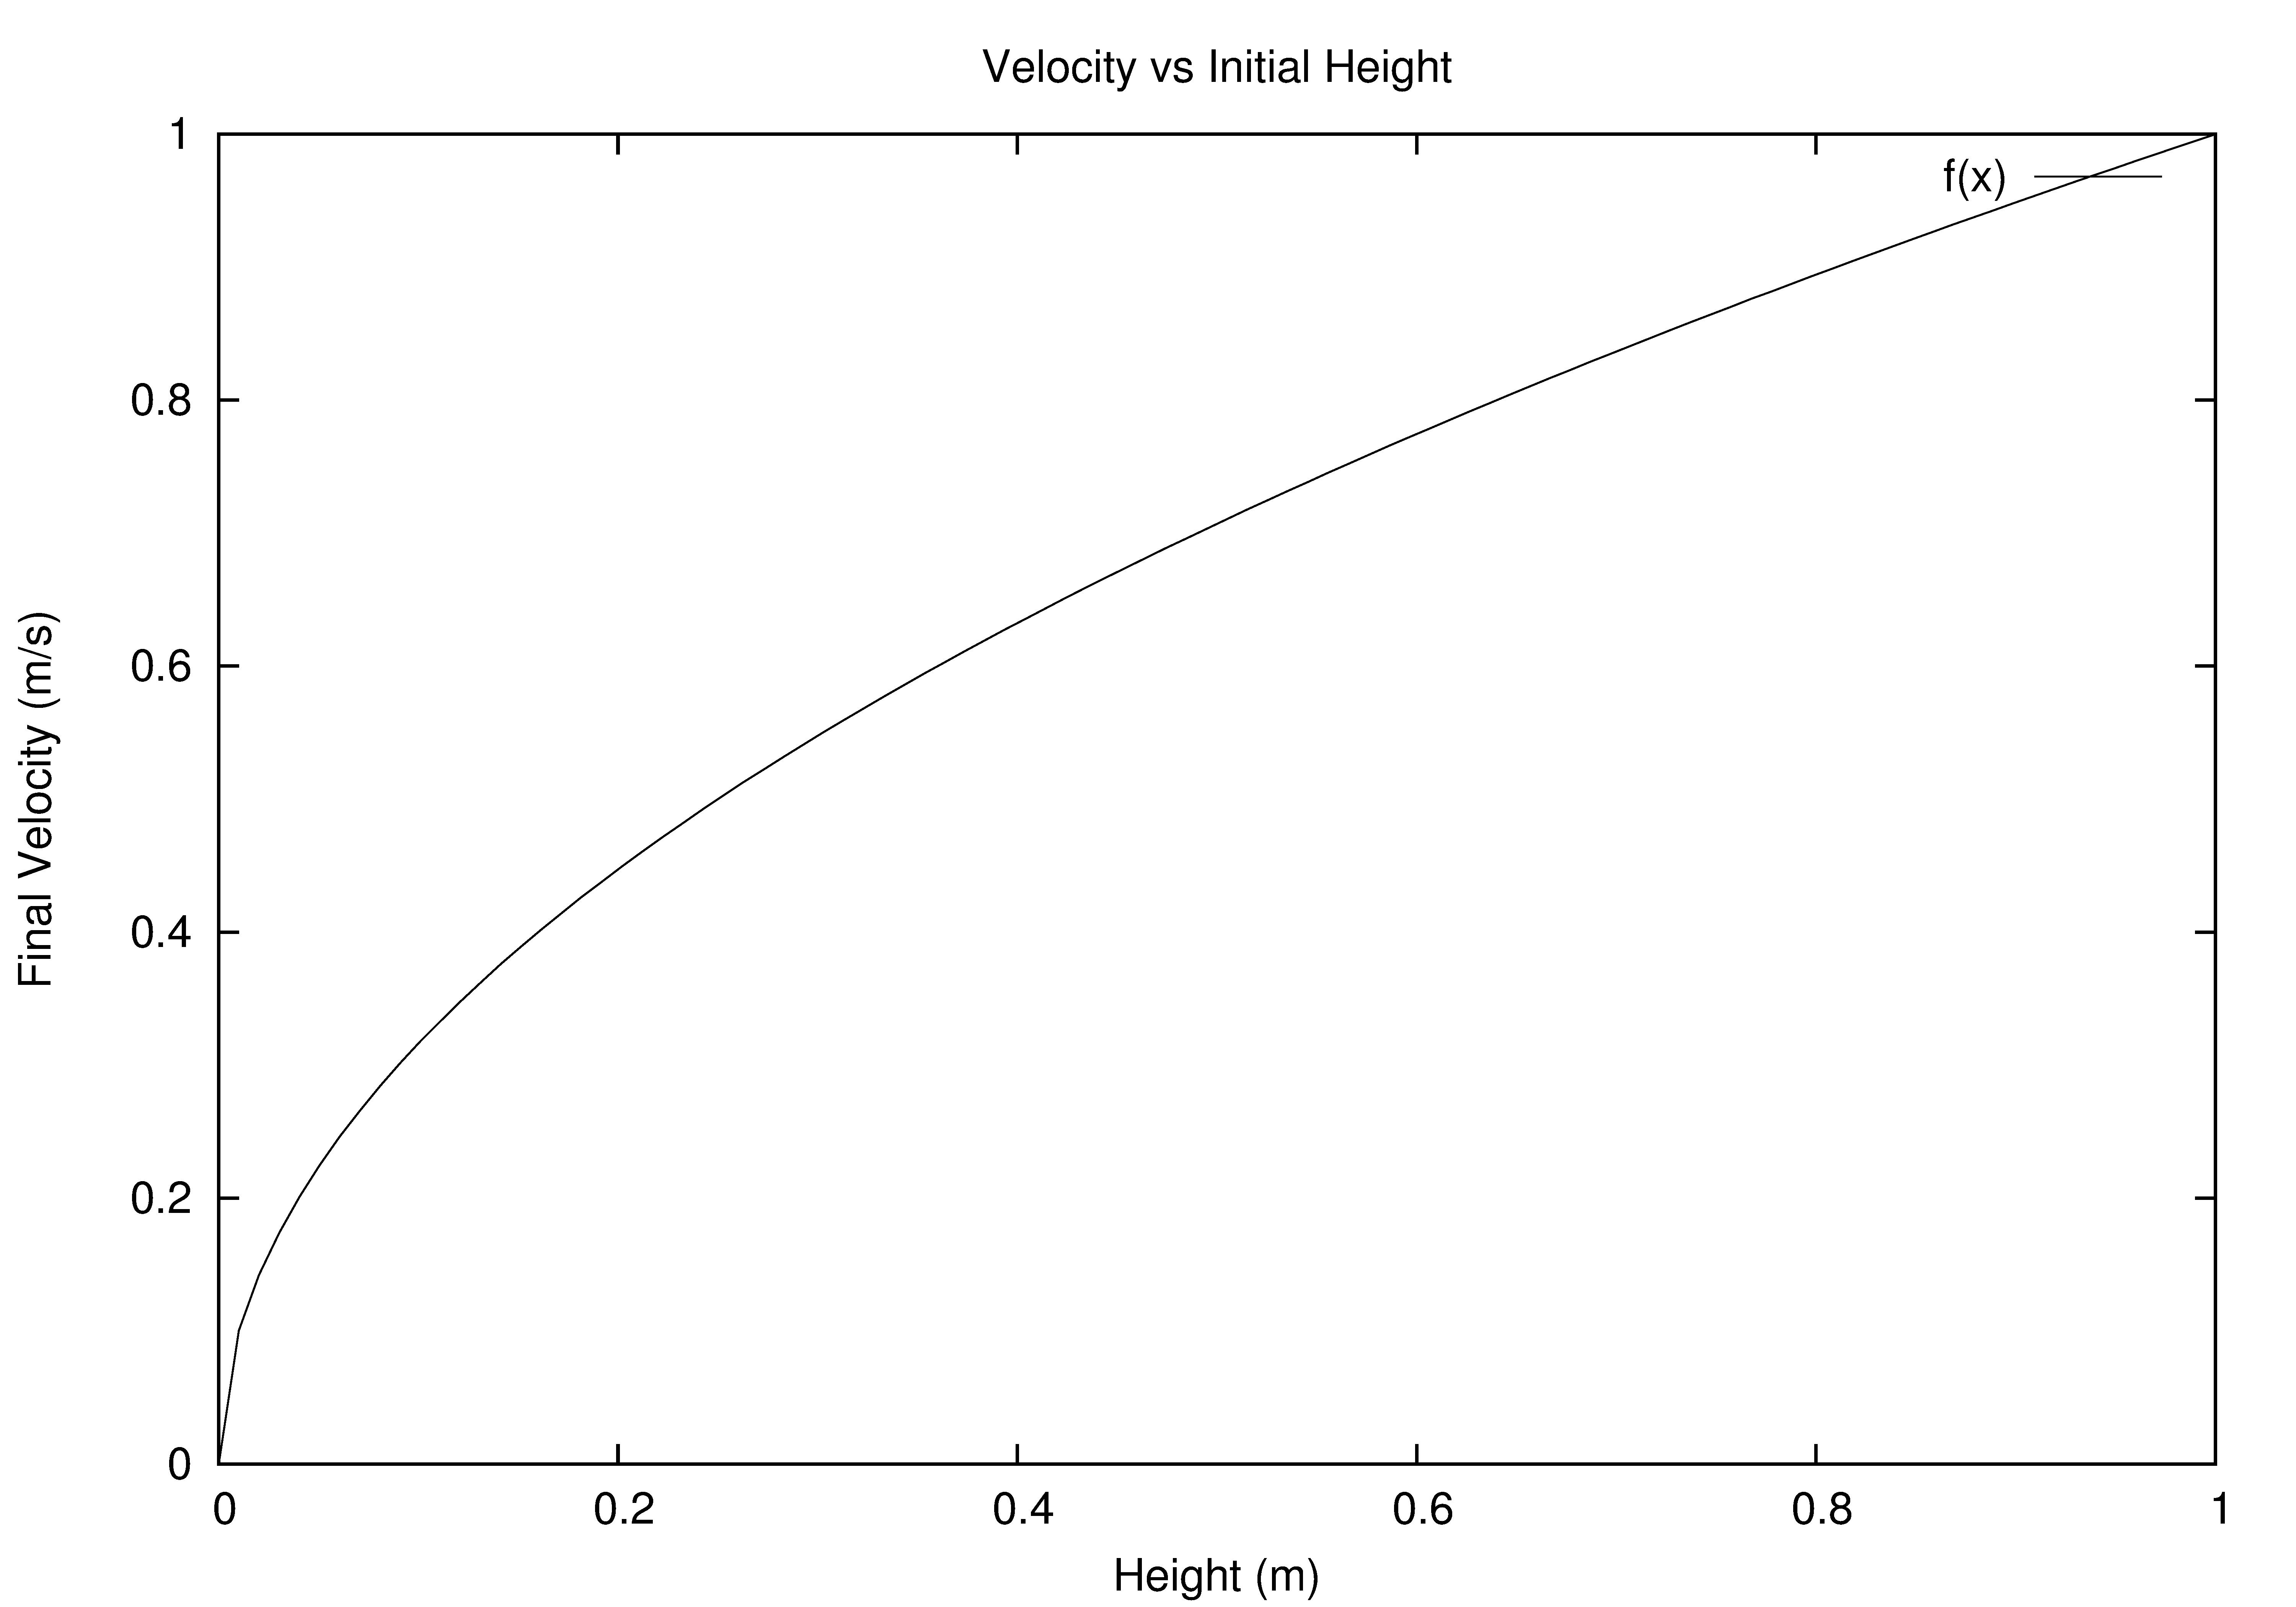
\includegraphics[scale=0.41]{h.png}
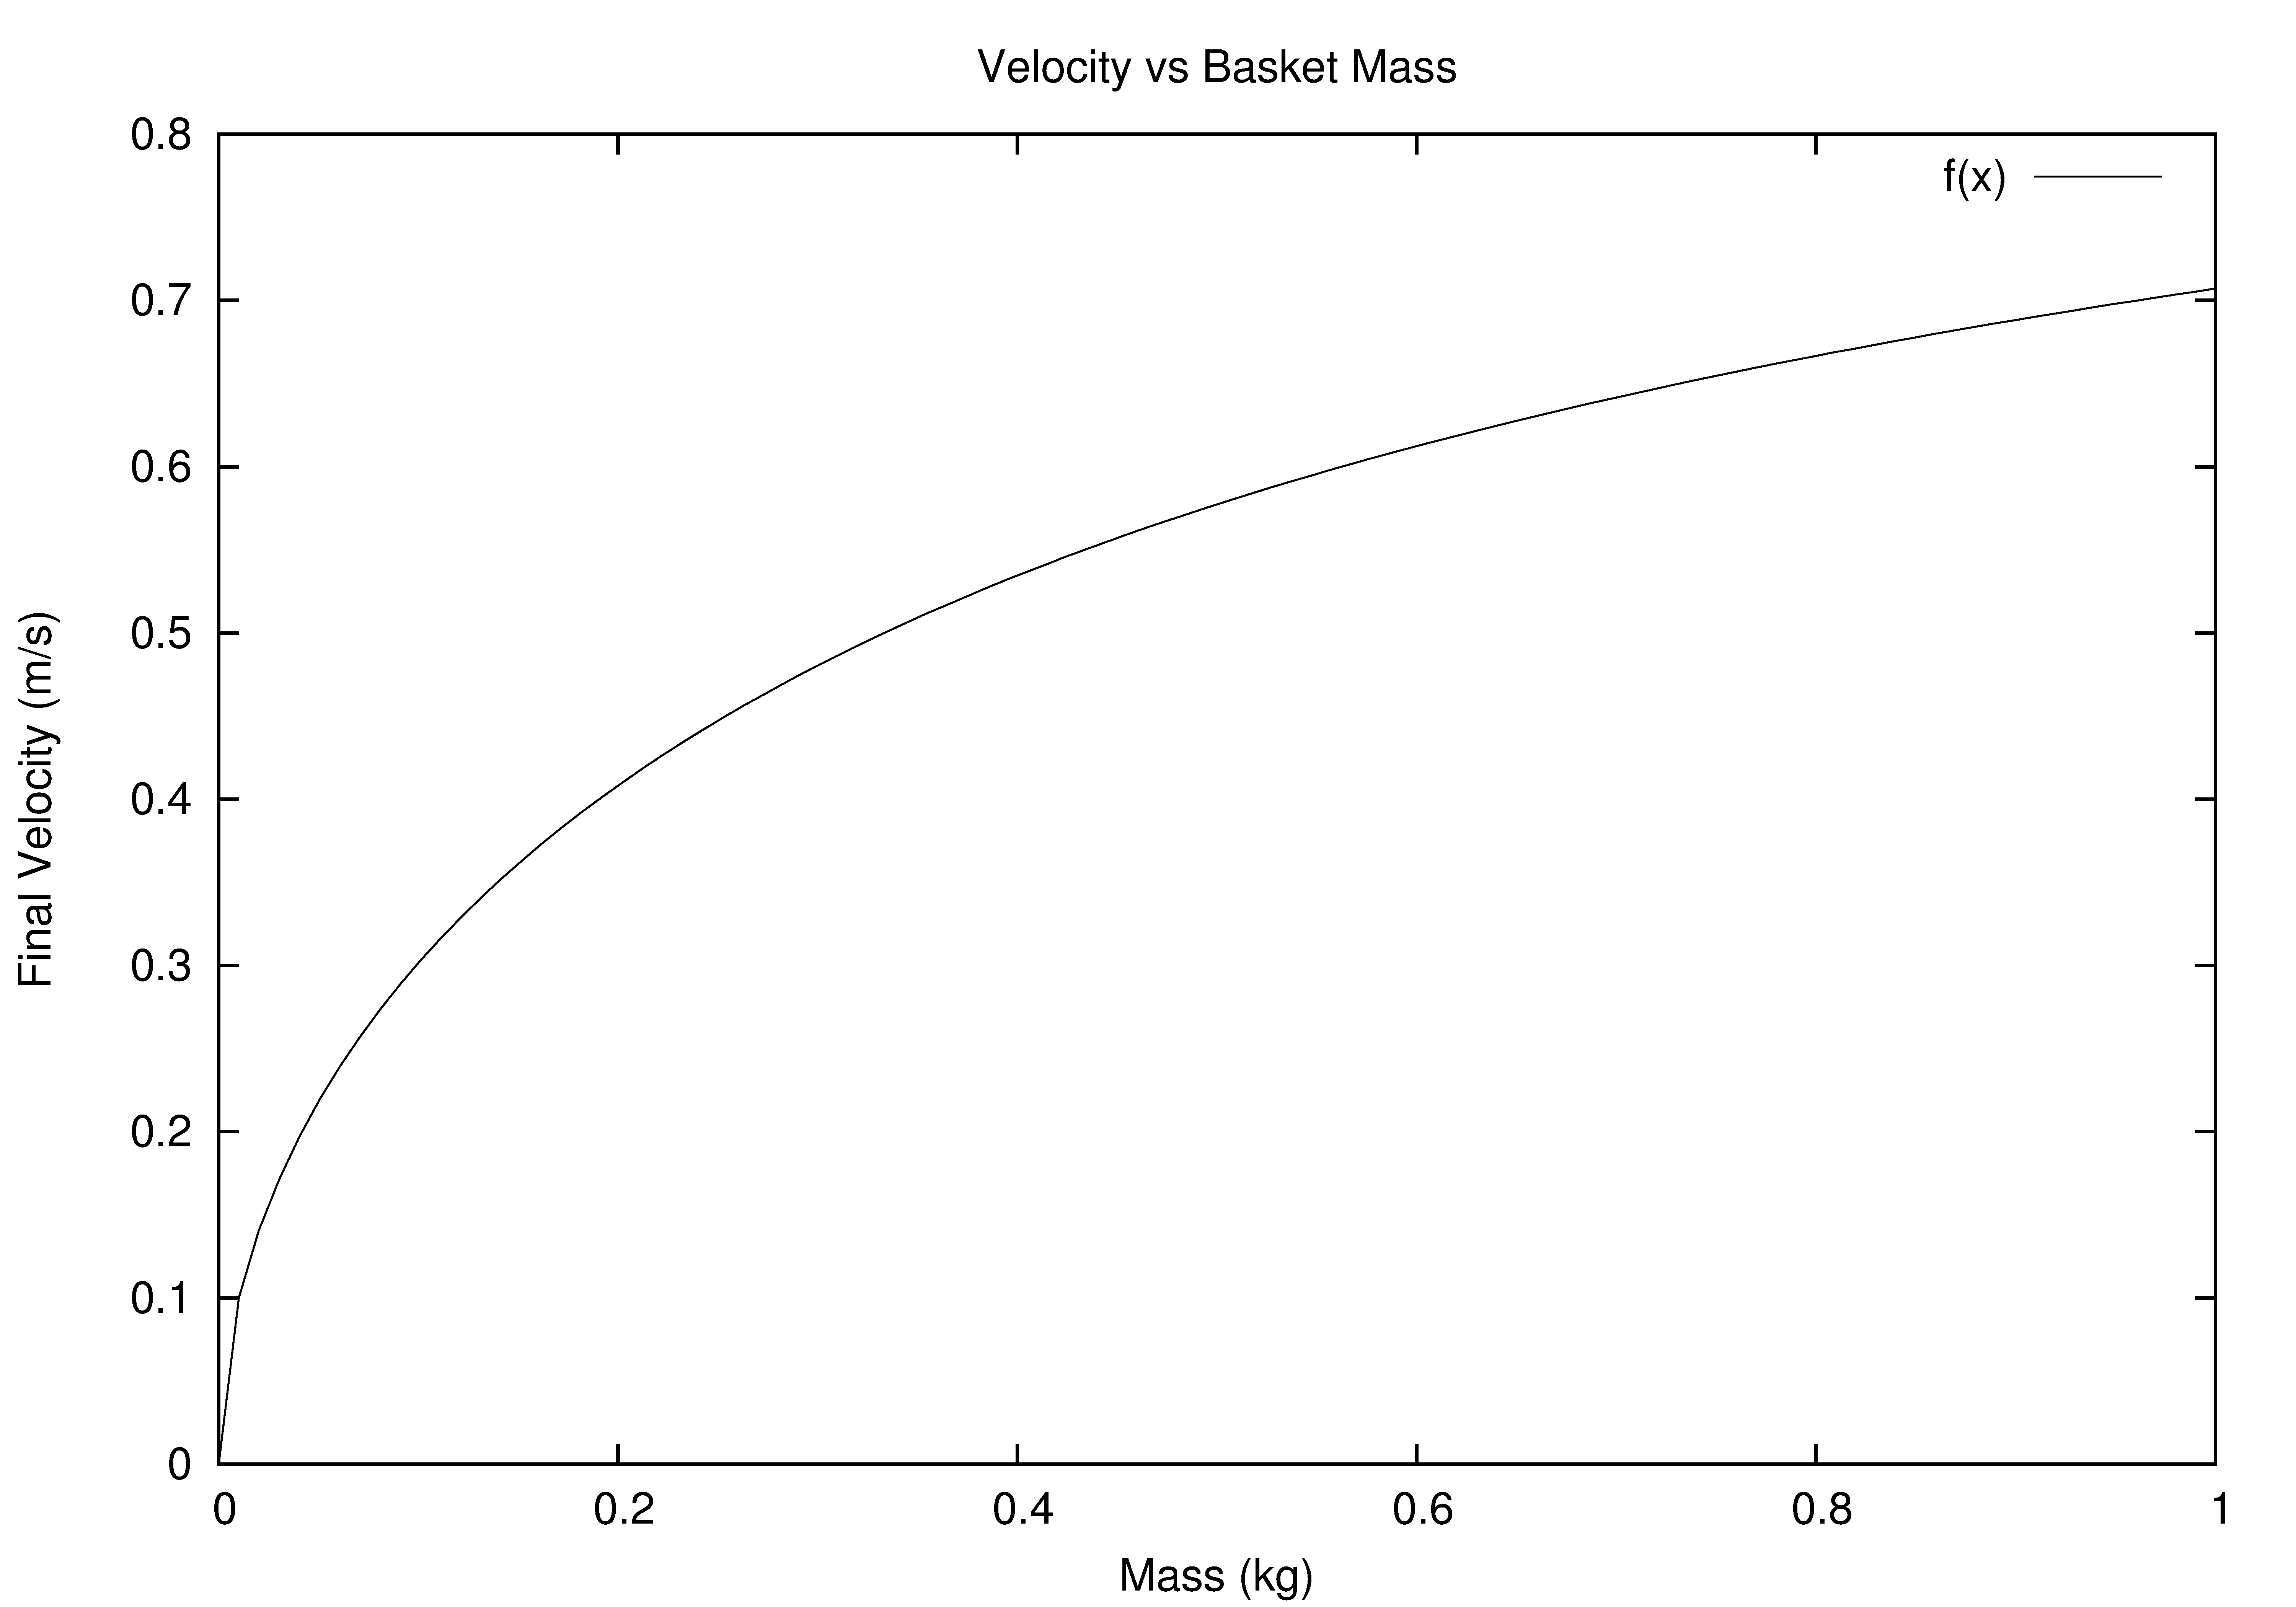
\includegraphics[scale=0.41]{mb.png}
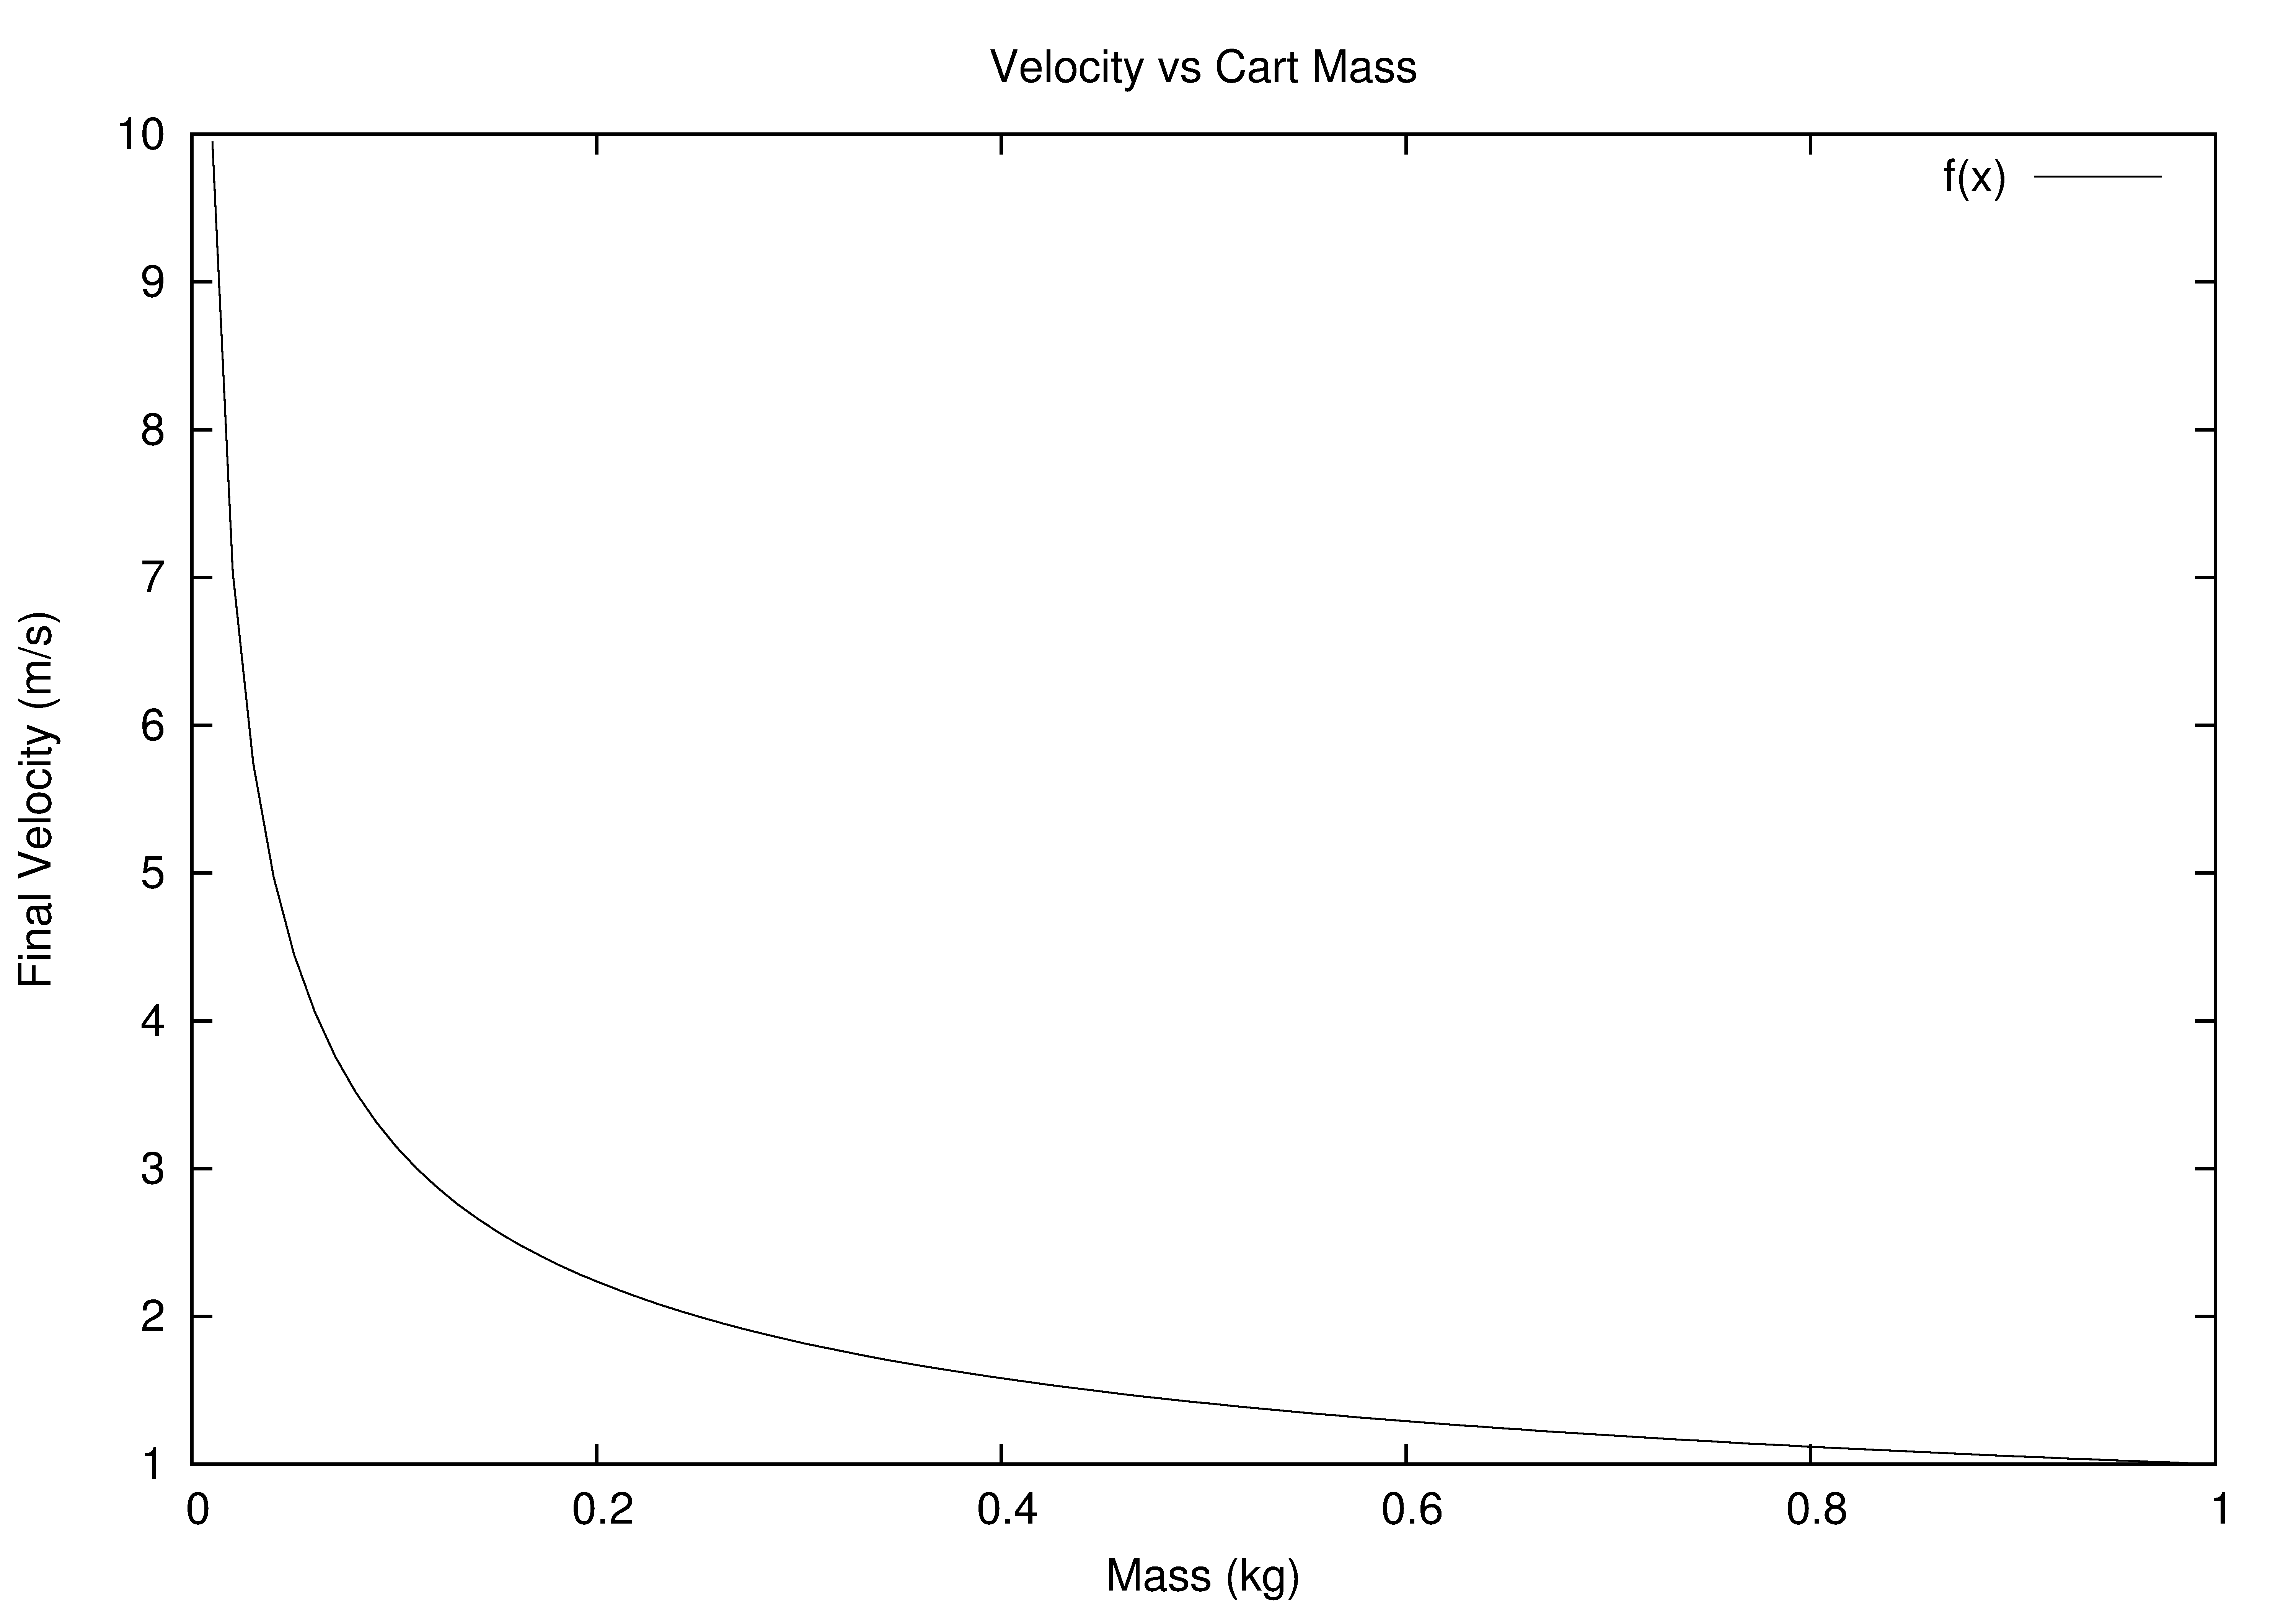
\includegraphics[scale=0.41]{mc.png}
\newline\newline
Above we we see that an increase in either height or \(m_b\) yields an increase in \(v_f\) and that an increase in \(m_c\) will yield a decrease in \(v_f\).
\section{Procedure}
Three trials of this experiment were performed. At the start of each trial, values for \(h\), \(m_b\) and \(m_c\) were selected such that (A) there was variance in these numbers between trials and (B) the cart would move at a velocity where enough data points could be recorded. Also, the camera was set up so the motion of the cart would avoid the edges of the frame where distortion is highest and that the frame include a meter stick a few centimeters from the cart's path for Motionlab calibration. Next, the experiment was set up as shown in \textit{Figure 1}, and the system was constrained from motion by holding the cart. Finally, the constraint was removed from the system  and the resulting motion was recorded using the camera. Motionlab was then used to generate points containing the time and position of the cart at that time. This is done by calculating the change in position (using the meter stick as a reference/calibration object) and the change in time between frames (\(\frac{1}{30}\) second). The data for each trial was then fitted with two functions, one quadratic during the period where the system was accelerating, and the second linear for the period where the cart was moving at a constant velocity \(v_f\). This was done by using quadratic regression for the former and least-square linear regression for the latter. Last, the data points and best-fit functions for each trial were plotted using Gnuplot.
\section{Data}

For each trial, the original postion plot from Motionlab will be included followed by an improved plot generated using Gnuplot including the position functions found using regression algorithms and the data points. After the plots, the equations of the functions, coefficients of determination (from the regression algorithm) and initial conditions for each trial will be listed. 
\newline\newline
\textbf{Trial 1}
\newline\newline
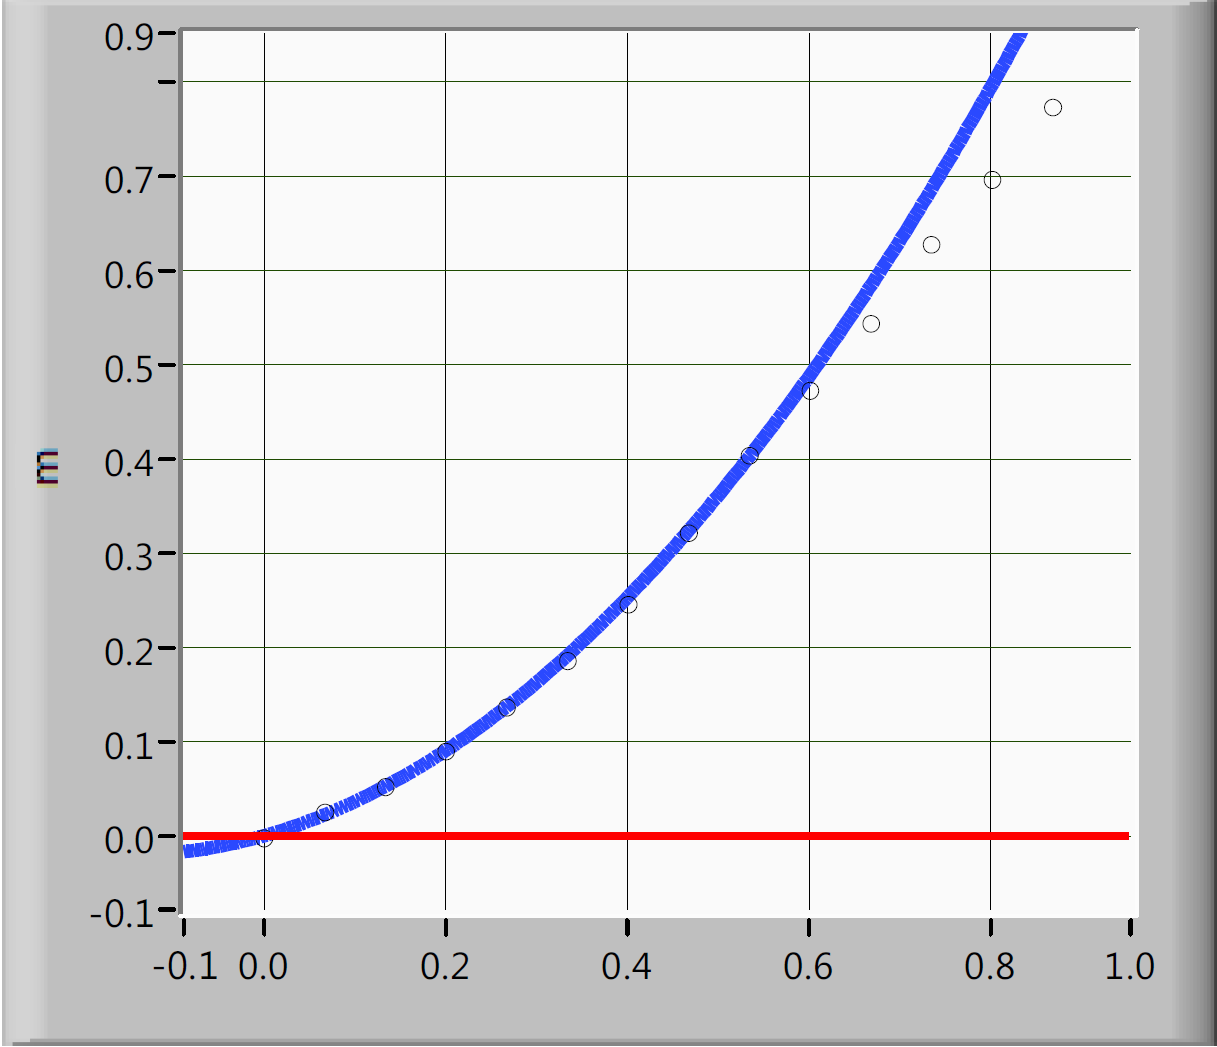
\includegraphics[scale=0.43]{t1p.PNG}
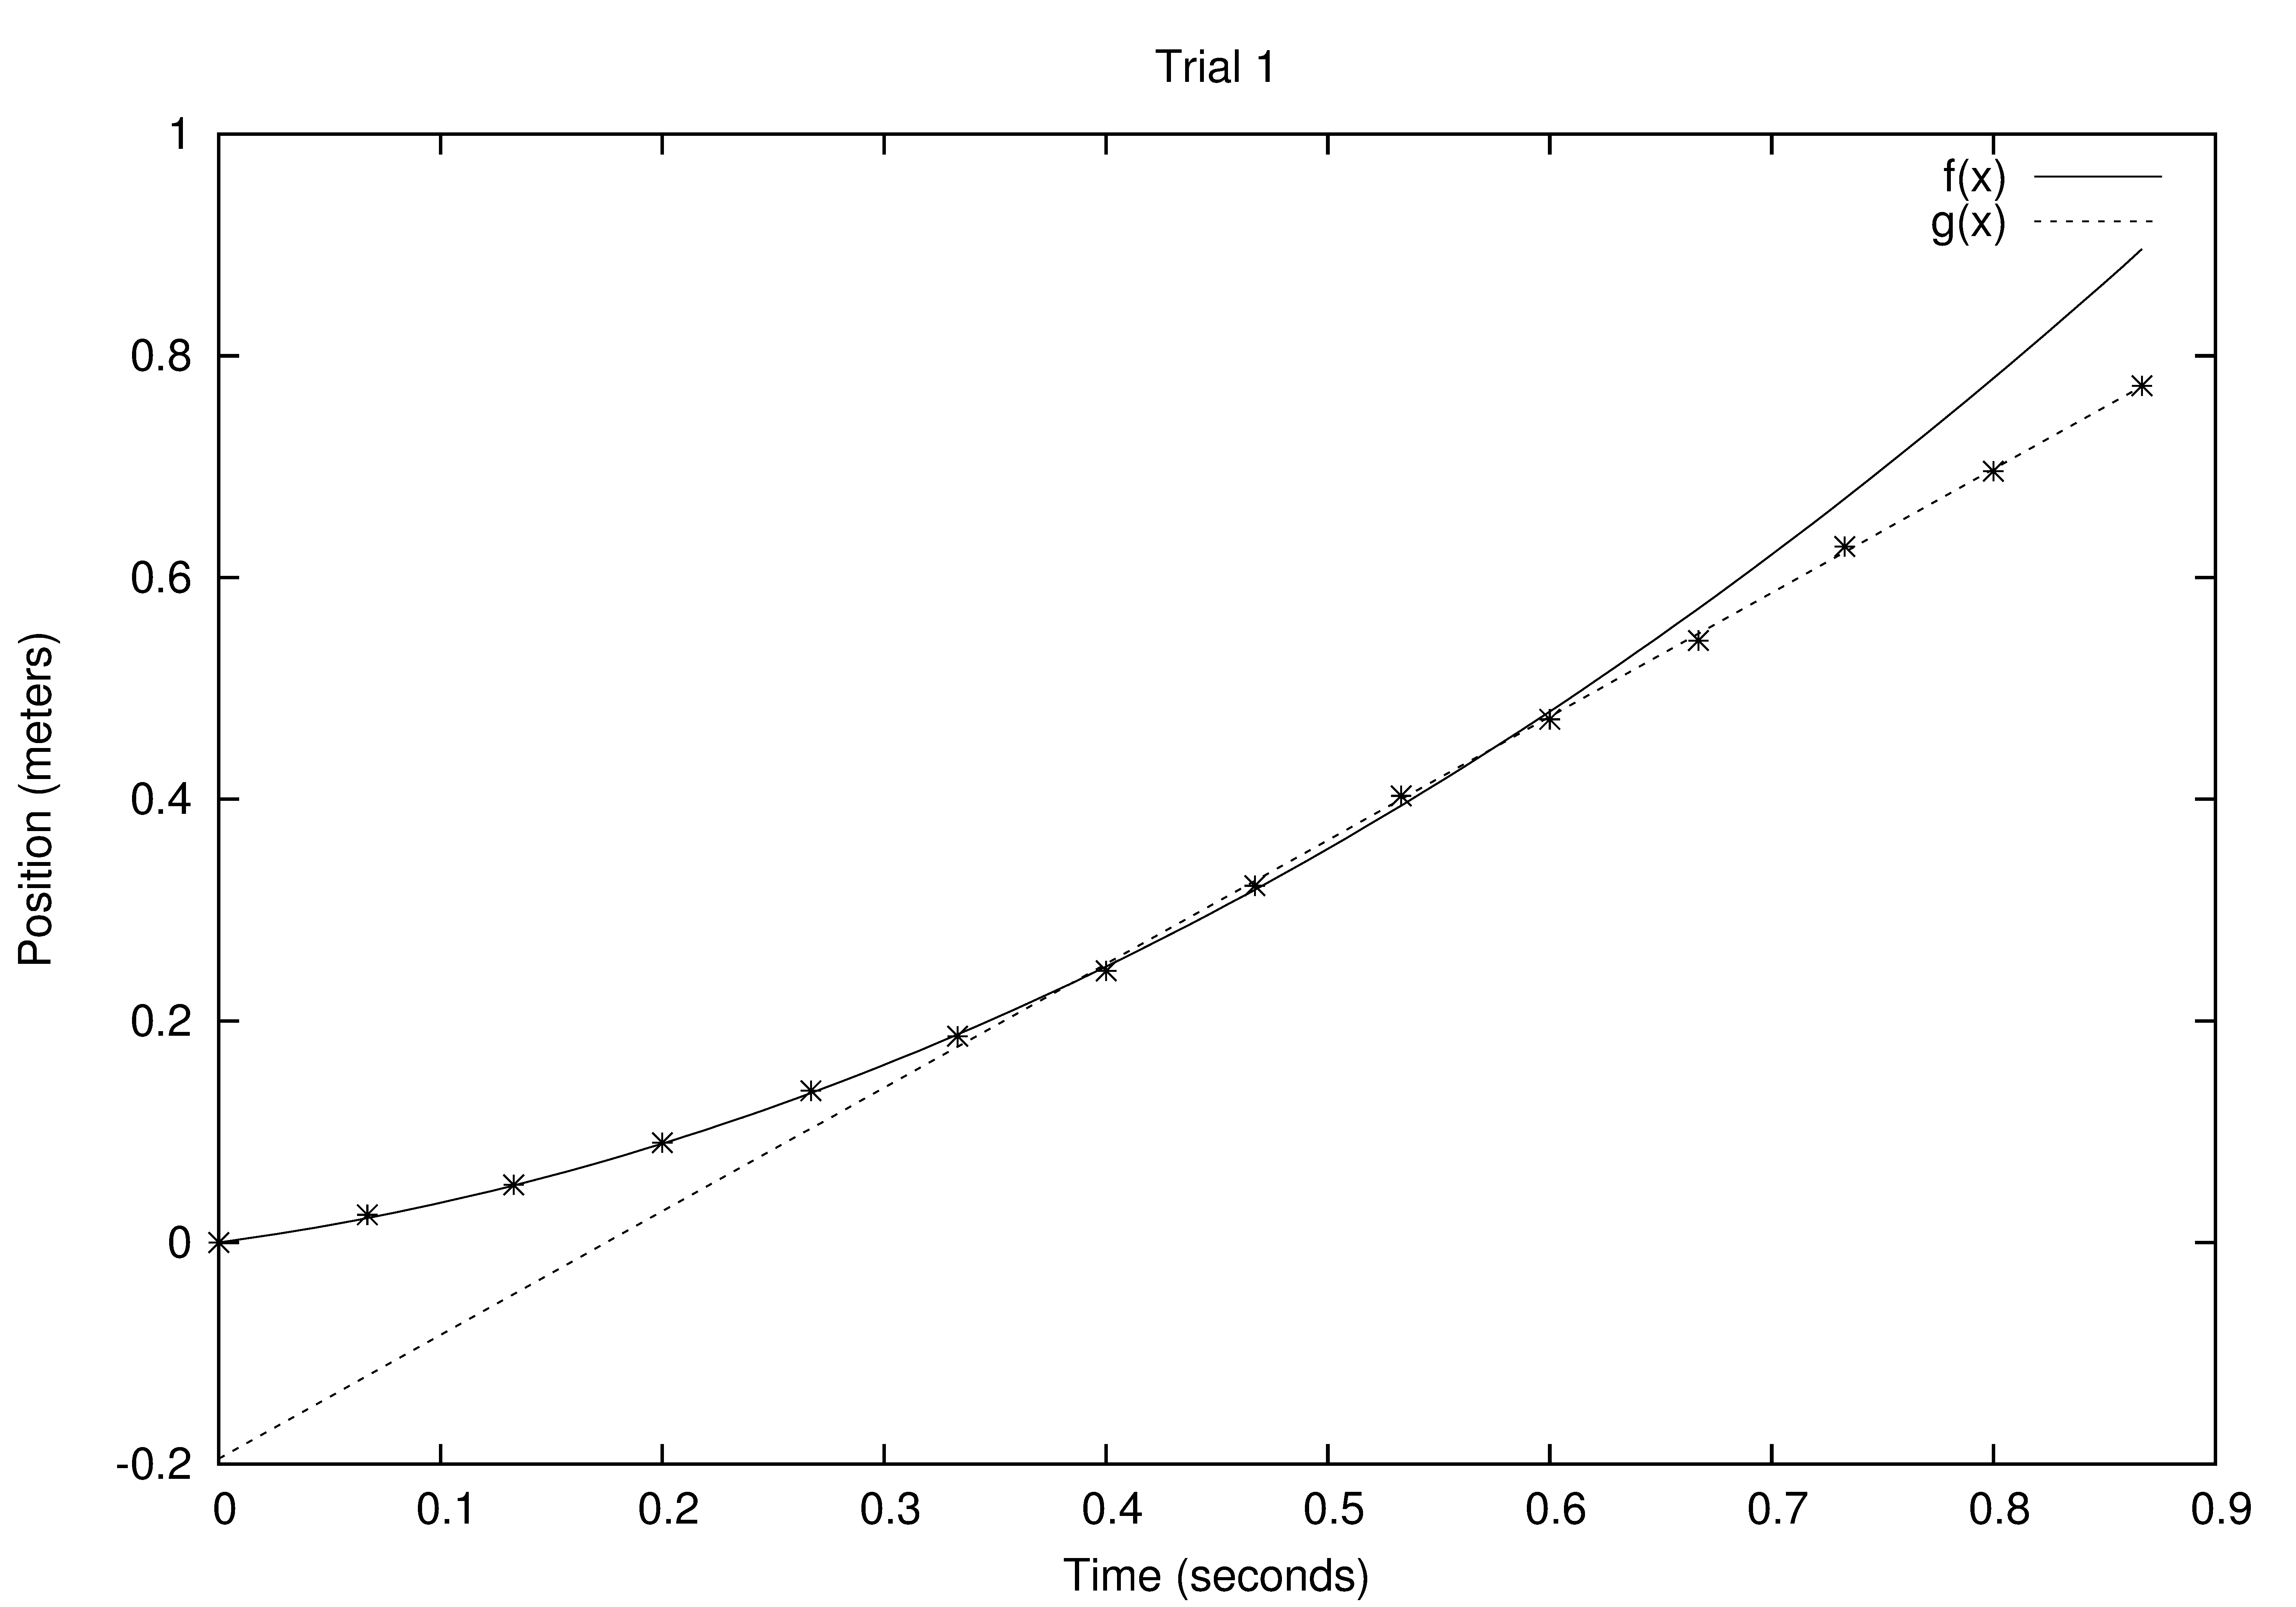
\includegraphics[scale=0.7]{1.png}
\textit{Left: Figure 2.} Motionlab Position v. Time plot \textit{Right: Figure 3.} Plot with regression lines
\newline

\(f(t) = 0.881t^2 + 0.270t\), solid line in \textit{Figure 3}.

\(R^2\) = 0.99944

\(g(t) = 1.116t - 0.195\), dashed line in \textit{Figure 3}.

\(r^2\) = 0.99913

\(h\) = .394 \(\pm\) 0.005 m, \(m_b\) = 0.050 kg, \(m_c\) = 0.252 kg
\newline\newline
\textbf{Trial 2}
\newline\newline
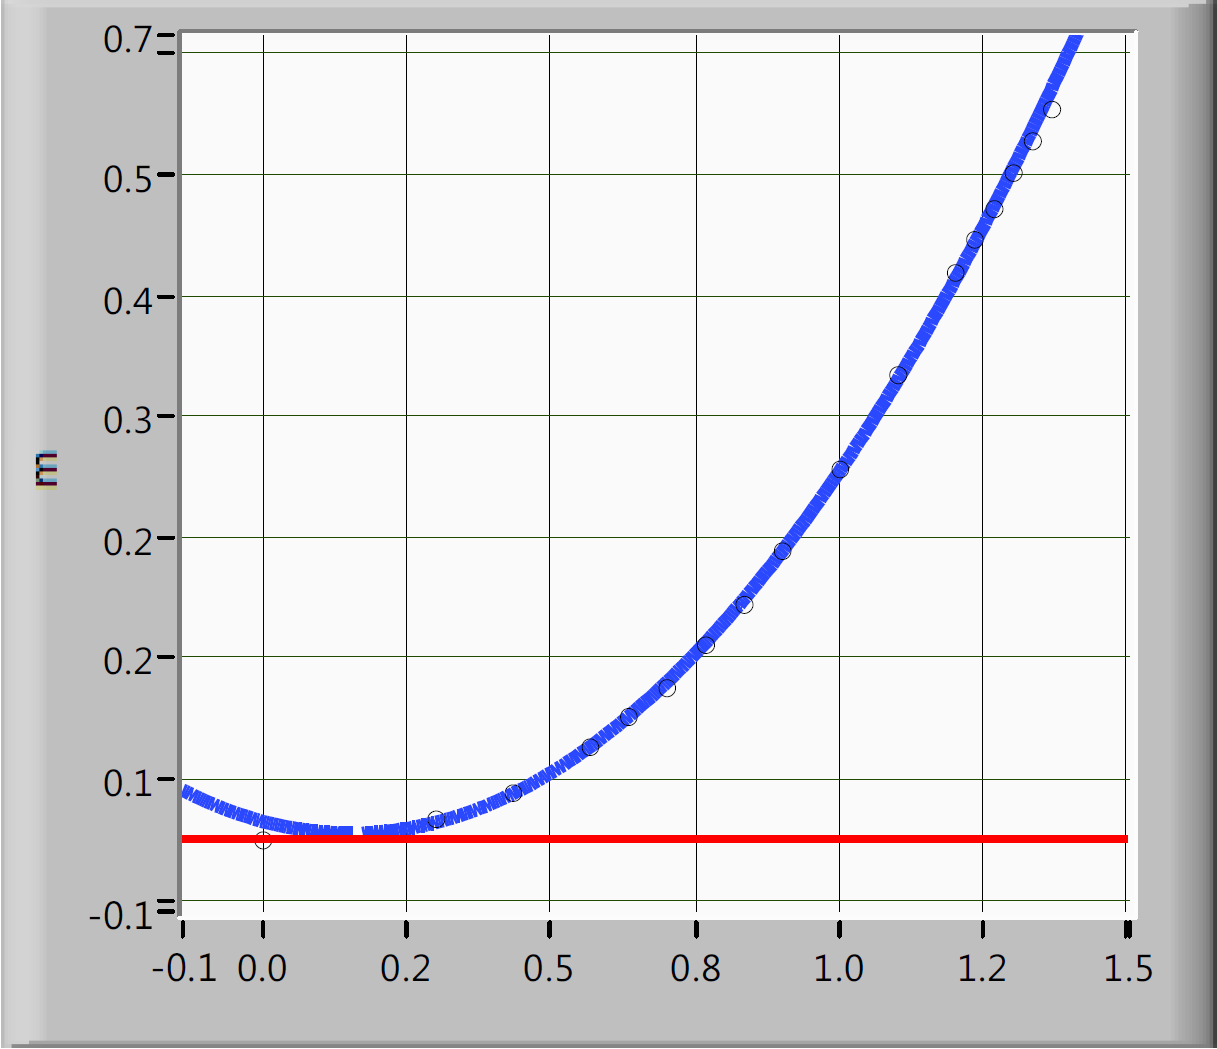
\includegraphics[scale=0.43]{t2p.PNG}
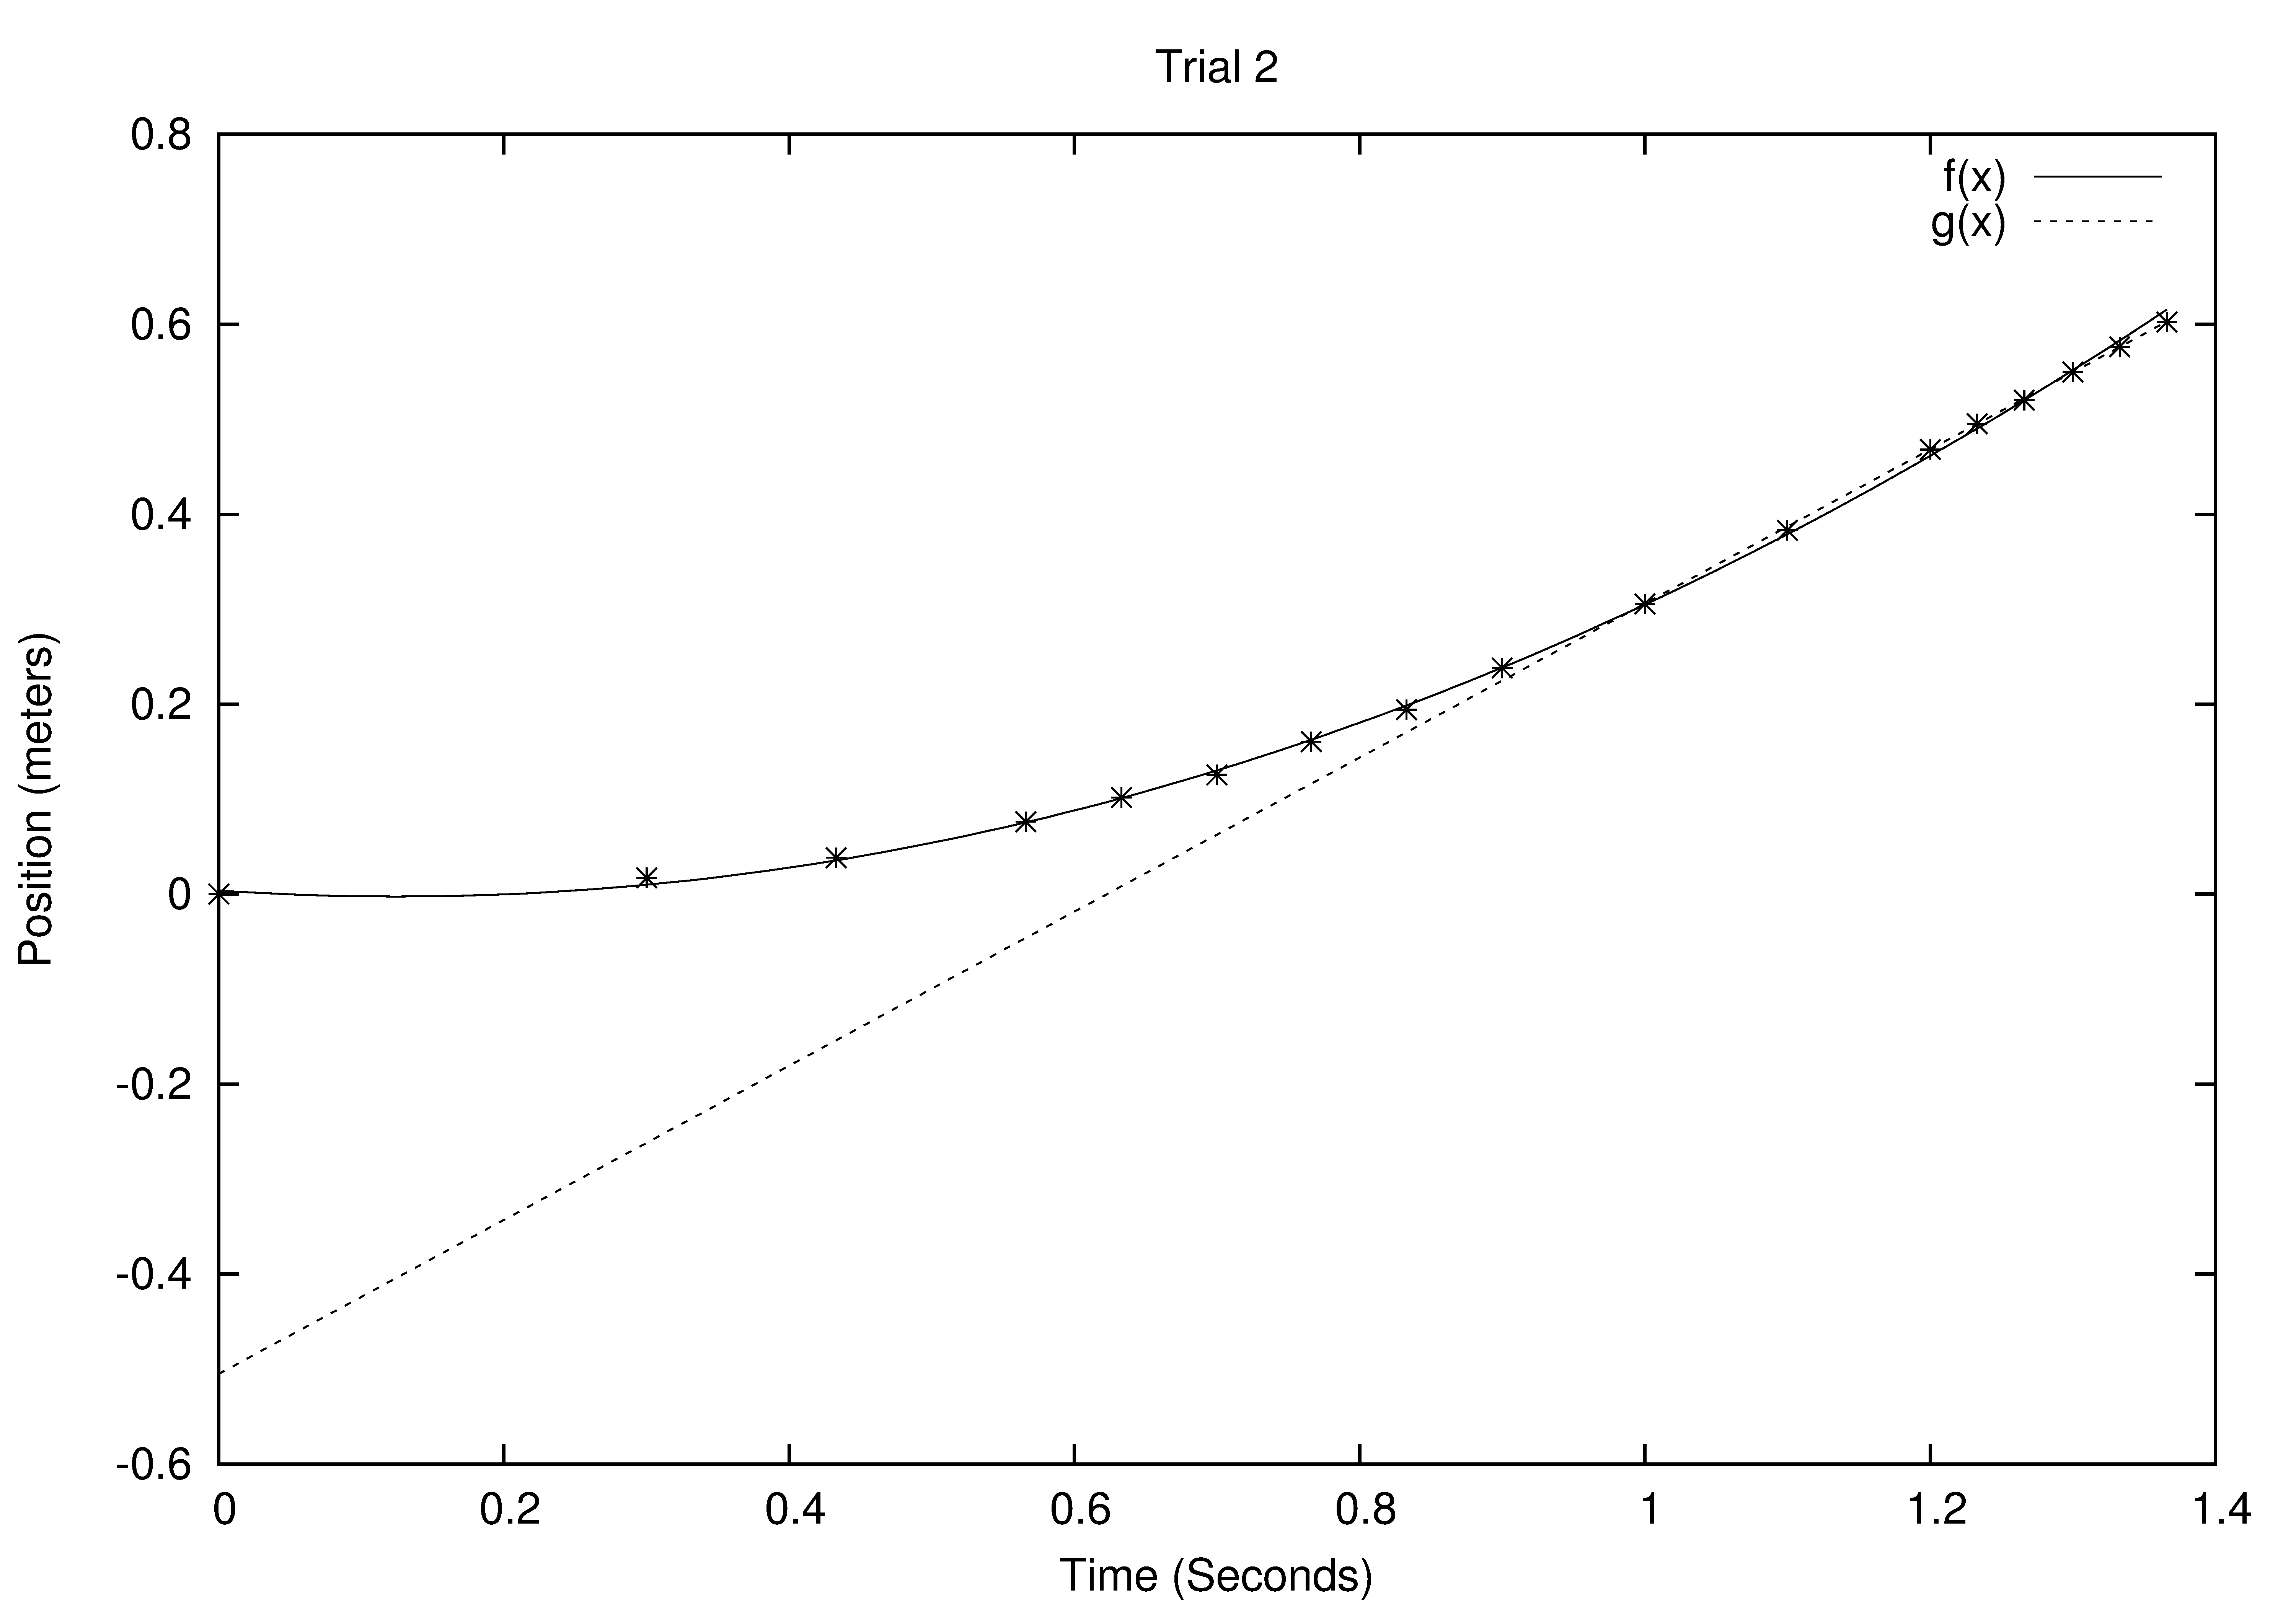
\includegraphics[scale=0.7]{2.png}
\newline
\textit{Left: Figure 4.} Motionlab Position v. Time plot \textit{Right: Figure 5.} Plot with regression lines
\newline

\(f(t) = 0.407t^2 - 0.100t + 0.0038\), solid line in \textit{Figure 5}.

\(R^2\) = 0.99906

\(g(t) = .811t - 0.505\), dashed line in \textit{Figure 5}.

\(r^2\) = 0.99978

\(h\) = 0.394 \(\pm\) 0.005 m, \(m_b\) = 0.050 kg, \(m_c\) = 0.502 kg
\newline\newline
\textbf{Trial 3}
\newline\newline
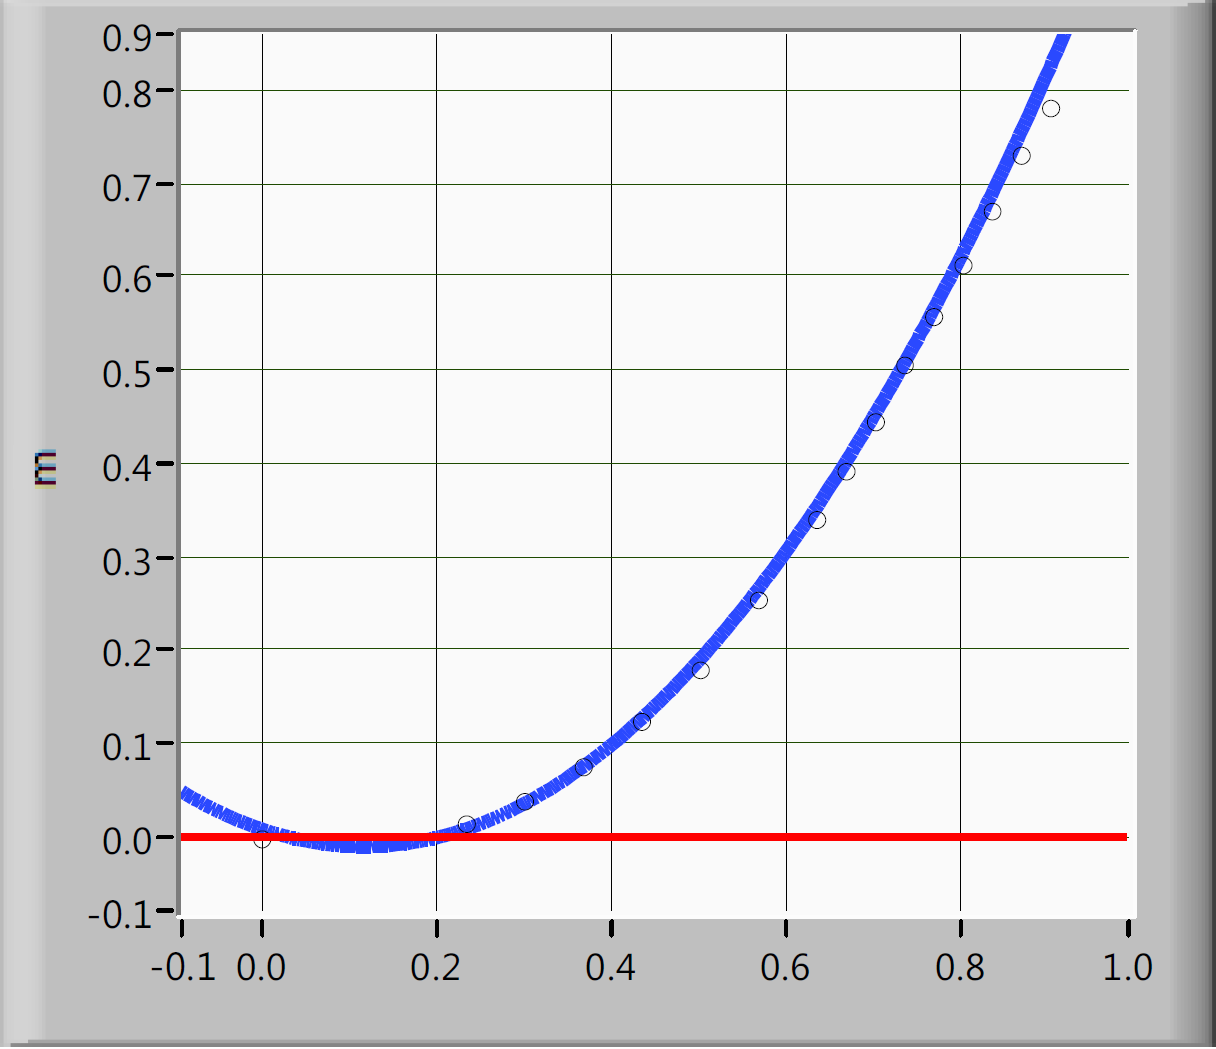
\includegraphics[scale=0.43]{t3p.PNG}
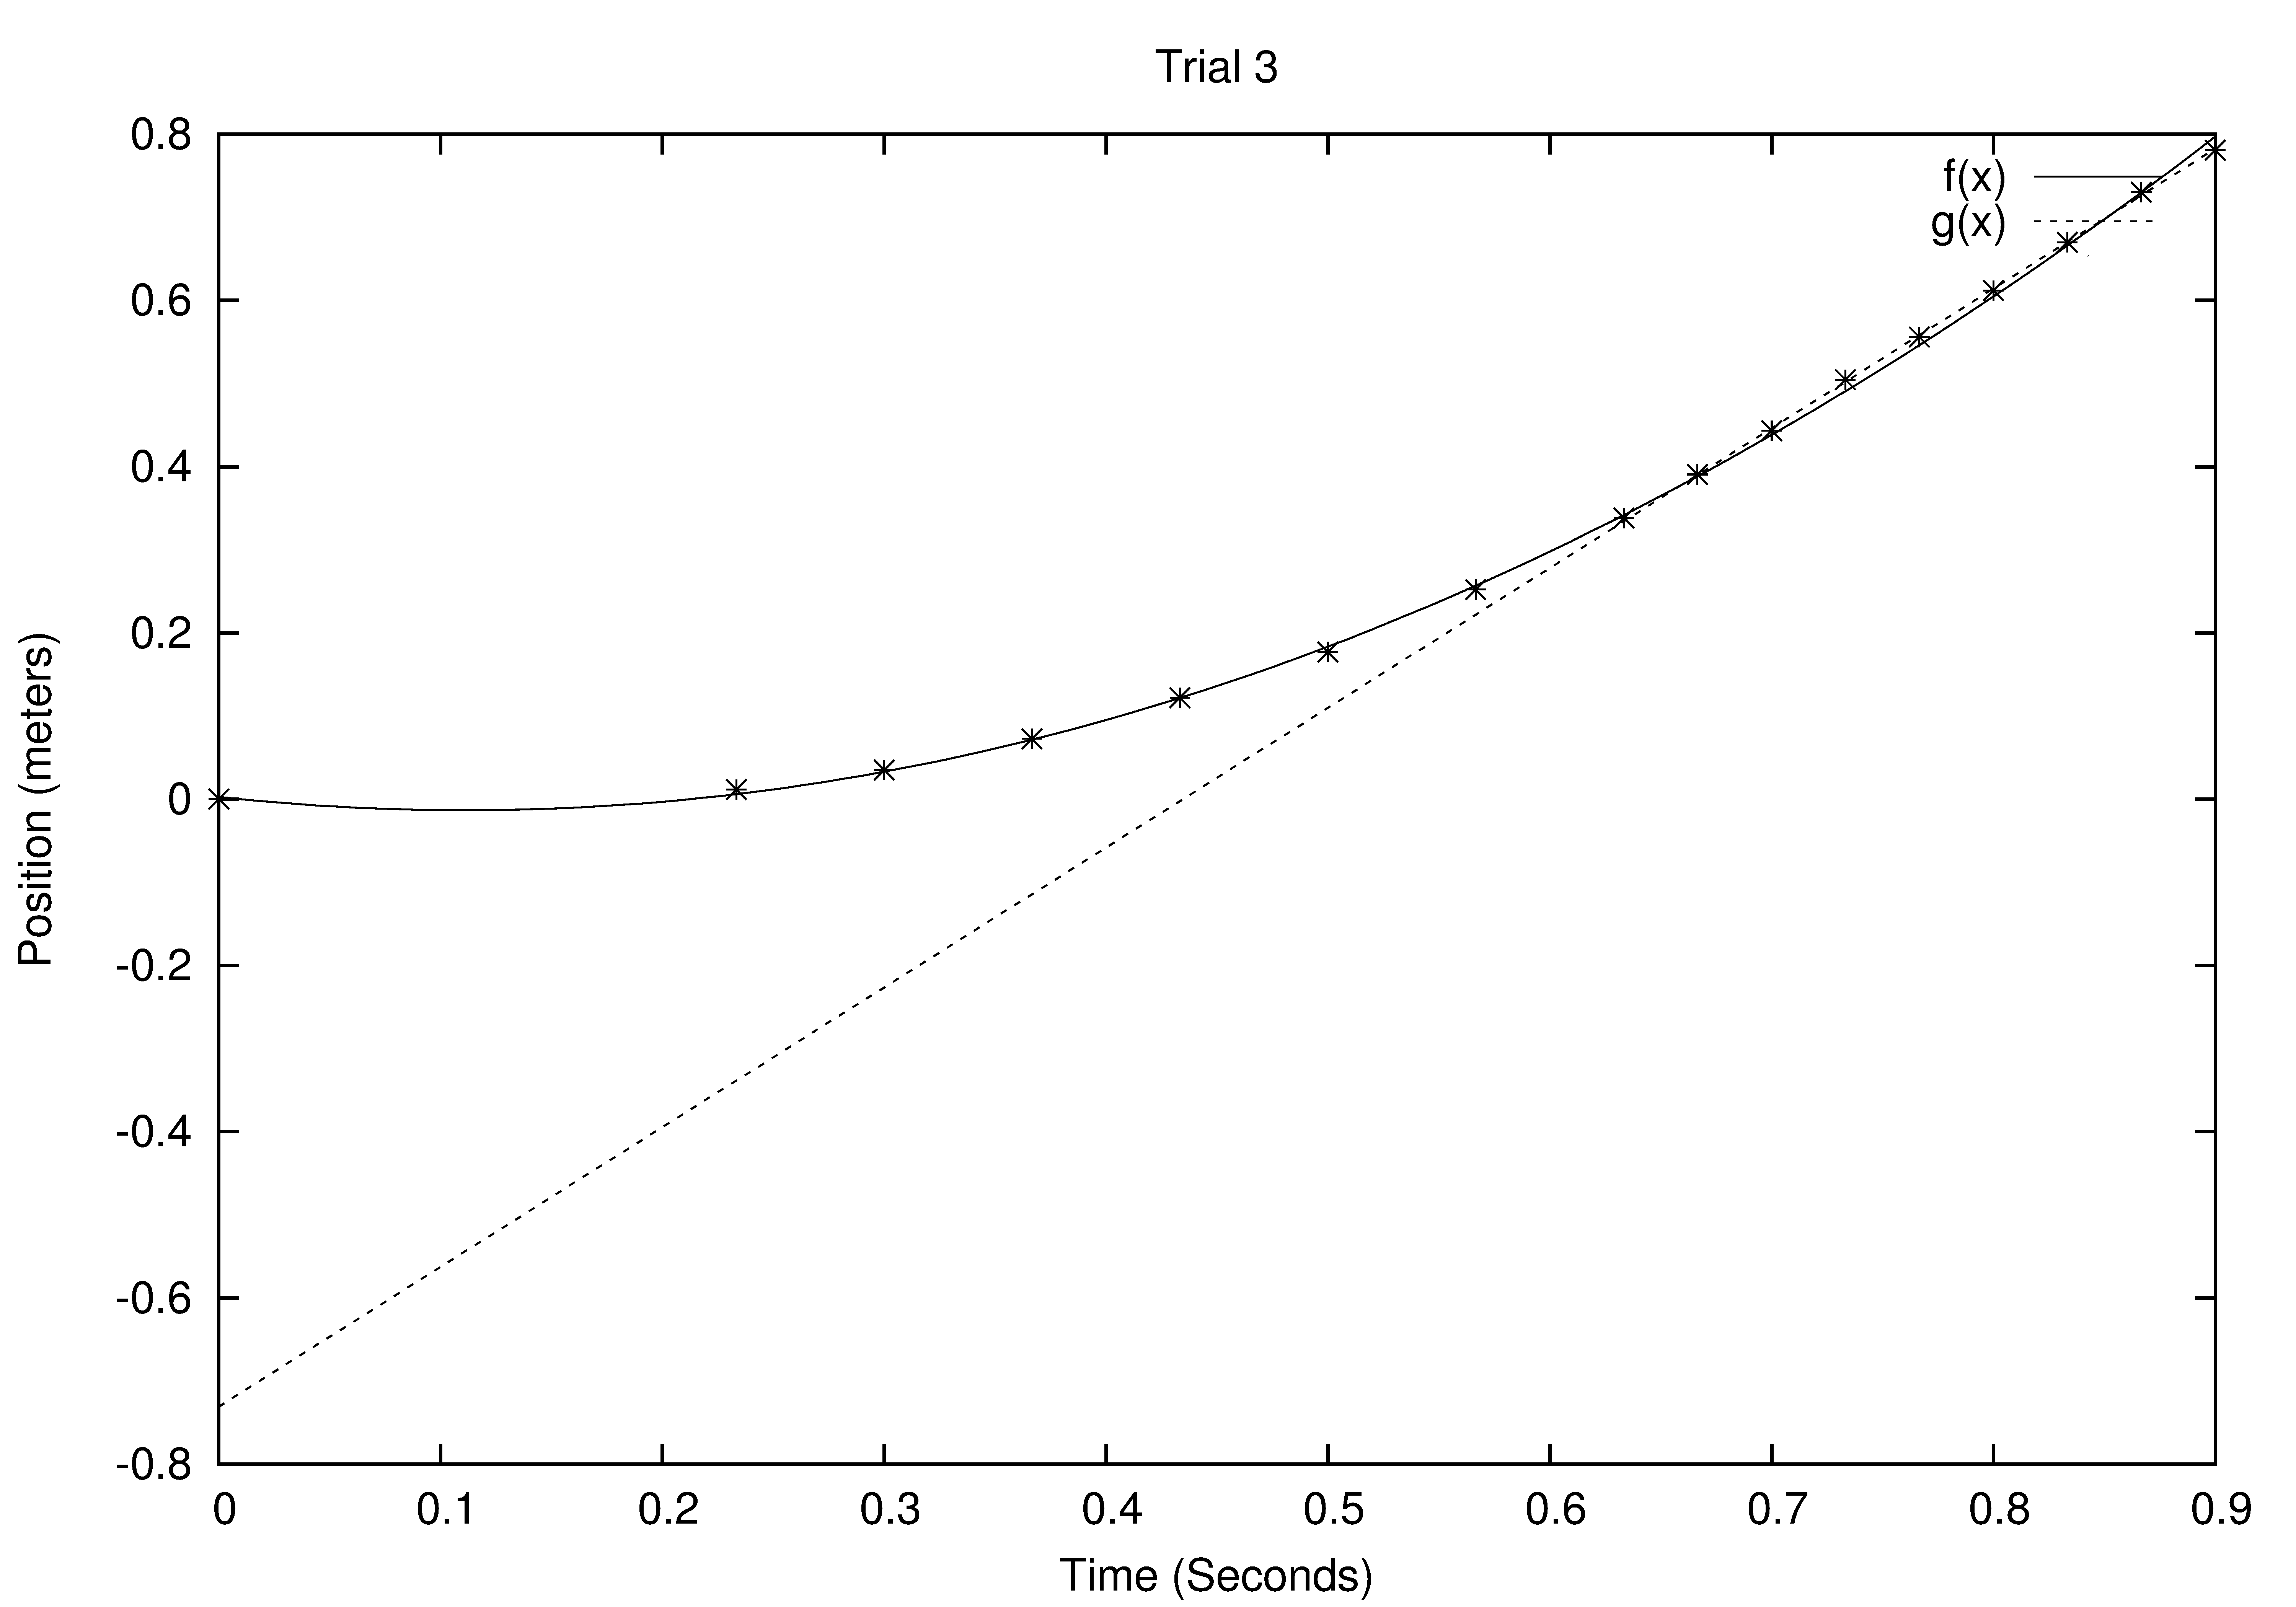
\includegraphics[scale=0.7]{3.png}
\textit{Left: Figure 6.} Motionlab Position v. Time  \textit{Right: Figure 7.} Plot with regression lines
\newline

\(f(t) = 1.303t^2 - 0.290t + 0.003\), solid line in \textit{Figure 7}.

\(R^2\) = 0.99937

\(g(t) = 1.682t - 0.731\), dashed line in \textit{Figure 7}.

\(r^2\) = 0.99941

\(h\) = 0.49 \(\pm\) 0.005 m, \(m_b\) = 0.100 kg, \(m_c\) = 0.252 kg

\newpage
\section{Analysis}
In order to show that the predicted equation for \(v_f\) is valid, we must simply test several different scenarios with difrernt initial conditions for each \(h\), \(m_b\) and \(m_c\). If our predictions for \(v_f\) and experimental data for \(v_f\) agree, then it can be concluded that the equation is indeed valid.
\newline\newline
\textbf{Predictions}
\newline
\textit{Table 1} below lists the initial conditions for each trial (\(h\), \(m_b\) and \(m_c\)). Also listed will be the expected final velocity \(v_{f,e}\) and expected acceleration \(a_e\) found using the equations for \(v_f\) and acceleration derived in the \textit{Prediction} section.
\newline\newline
\textit{Below: Table 1.} Predictions.
{\renewcommand{\arraystretch}{1.2}
\begin{table}[h]
\hspace{0.7in}
\begin{tabular}{l|l|l|l|l|l}
Trial & \(h\) & \(m_b\) & \(m_c\) & \(a_e\) & \(v_{v,e}\)\\
1 & 0.394 \(\pm\) .005 m & 0.050 kg & 0.252 kg & 1.623 \(\frac{m}{s^2}\) & 1.131 \(\pm\) 0.0075 \(\frac{m}{s}\)\\
2 & 0.394 \(\pm\) .005 m & 0.050 kg & 0.502 kg & 0.888 \(\frac{m}{s^2}\) & 0.837 \(\pm\) 0.0051 \(\frac{m}{s}\)\\
3 & 0.490 \(\pm\) .005 m & 0.050 kg & 0.252 kg & 2.785 \(\frac{m}{s^2}\) & 1.652 \(\pm\) 0.0210 \(\frac{m}{s}\)\\                 
\end{tabular}
\end{table}
\newline
}
\textbf{Experimental Velocity}
\newline
The velocity of an object over time can be found as the derivative of the function representing its position with respect to time. Mathematically: 
\begin{equation}
\frac{dx(t)}{dt} = v(t) 
\end{equation}
So, to determine the actual final velocity \(v_f\) of the cart after the basket (\(m_b\)) hits the ground, all that has to be done is take the derivative with respect to time of the function representing the carts position after the cart hits the ground. That function is represented as g(x) in each trial in the \textit{Data} section. Below is a table containing the experimental values for \(v_f\) of each trial found using the above method:
\newline\newline
\textit{Table 2.} Experimental final velocities.
{\renewcommand{\arraystretch}{1.2}
\begin{table}[h]
\hspace*{2.4in}
\begin{tabular}{ll}
Trial \hspace{12pt} &\hspace{12pt} Final Velocity\\
\hspace{10pt}1       & \hspace{30pt}1.116 \(\frac{m}{s}\)  \\   
\hspace{10pt}2       & \hspace{30pt}0.811 \(\frac{m}{s}\)   \\  
\hspace{10pt}3       & \hspace{30pt}1.682 \(\frac{m}{s}\)   \\  
\end{tabular}
\end{table}
}
\newline
\textbf{Comparison and Validation of Prediction}%
\newline\newline
\textit{Below: Table 3.} Contains the predicted and experimental values for \(v_f\) for each trial.
{\renewcommand{\arraystretch}{1.2}
\begin{table}[h]
\hspace*{1.2in}
\begin{tabular}{lll}
Trial  \hspace{.5in} & \hspace{0.15in} Predicted \(v_f\)\hspace{.5in} & Experimental \(v_f\)\\
\hspace{.14in}1&\hspace{0in} 1.131 \(\pm\) 0.0075 \(\frac{m}{s}\)& \hspace{0.3in}1.116 \(\frac{m}{s}\) \\
\hspace{.14in}2&\hspace{0in} 0.837 \(\pm\) 0.0051 \(\frac{m}{s}\)& \hspace{0.3in}0.811 \(\frac{m}{s}\) \\
\hspace{.14in}3&\hspace{0in} 1.652 \(\pm\) 0.0210 \(\frac{m}{s}\)& \hspace{0.3in}1.682 \(\frac{m}{s}\)\\                 
\end{tabular}
\end{table}
\newline\newline
From the data in table 3, it is clear that the values for the predicted and the actual \(v_f\) are extremely close and consistent. Although the numbers do not overlap exactly given the experimental \(v_f\)'s minute tolerance ranges, the values found for each trial are within a couple hundreths of eachother, which is extremely close to the degree that any descrepencies can be accounted for by errors and inprecision of the equipment used (will be discussed in the below \textit{Error} subsection). The great level of closeness (agreement) between the experimental and predicted values suggests to a high level of certainty that our predicted equation is indeed valid and accurate in for this scenario.
\newline\newline
\textbf{Error}
\newline
There are several unaddressed sources of potential error in this experiment. The first source of potential error is due to lenticular distortion in the camera's image, particularly in the frame's extremities. To limit error from this effect, we avoided recording in frame's edges. Another source of error is due to poor calibration of length in Motionlab. To limit errors due to calibration, we used a large object (a meterstick) that extended over a large portion of the frame only a few centimeters away from the path of the cart (to reduce paralax errors). A third source of error is neglecting air resistance, which could have affected the carts velocity by decreasing it over time. One source of error that there is little control over is due to the camera's frame rate. Each frame is 1/30 of a second, and if the cart is moving sufficiently fast it can become blurred in the frame, making it hard to properly analyze the path of the object (which produces error). All of these errors cumulatively may have lead to some degree of error in our results, however the results from this experiment are within hundreths of meter per second, so the errors appear to be at a minimum. These errors, however, may explain the small difference of a few hundreths between the expected and experimental numbers.

\section{Conclusion}
Carts were attached by spring and pulley to a falling mass. The motion of the carts were analyzed to find the final velocity of the cart after the mass had fallen to the ground. A predicted equation for the cart's final velocity based on the scenario's initial conditions was then confirmed from data aquired in the experiment.
\newline\newline
The data aquired from this experiment confirms the predicted equation in the \textit{Prediction} section for a cart's final velocity in a scenario like that of \textit{Figure 1}. This assertion is made due to the agreeance between experimental and predicted data. 
\newline\newline
Based on this experiment, it seems that the final velocity of the cart is indeed dependent on height, mass of the cart and mass of the hanging basket. The relationship between each appears that increasing the height of the basket increases the final velocity (seen in trial 3), increasing the mass of the cart decreases the final velocity (seen in trial 2) and increasing the mass of the falling mass increases the final velocity (seen in trial 2), where trial 1 is the control.
\newline\newline
Lastly, the force of the string will always remain constant if the mass of the falling block remains constant, regardless of the mass of the cart. This is because if the block is a free falling mass, the force acting on it will always be equal to its mass times \(g\). Since it is the only force acting on the system and its mass is constant, the force will remain constant. 


\end{document}